\documentclass[paper=a4, fontsize=11pt]{scrartcl}
\usepackage{enumerate}
\usepackage{amsmath}
\usepackage{tikz}
\newcommand{\parens}[1]{ \left( #1 \right) }
\begin{document}
  \begin{center}
    STAT 221: Problem Set 2 \\
    Kevin Eskici and Willy Xiao \\
    Due: Oct 7, 2014
  \end{center}
  \begin{enumerate}[\text{Task }1:]
    \item Examine the Posterior \\

      Posterior is: $f(\mu, \sigma^2, \log{\vec{\theta}} | Y)$
      \begin{align*}
        f(\mu, \sigma^2, \log{\vec{\theta}} | Y) &\propto f(Y|\log{\vec{\theta}}) * f(\log{\vec{\theta}}|\mu, \sigma^2) * f(\mu, \sigma^2) \\
        &\propto \prod_{j=1}^{J}{
          \left[ \parens{
            \prod_{i=1}^N{
              e^{-w_je^{\log{\theta_j}}}\parens{w_je^{\log{\theta_j}}}^{Y_{ji}}
            }}
            * \frac{1}{\sigma}e^{
                                  \frac{-(\log{\theta_j}-\mu)^2}{2\sigma^2}
                                }
            * \frac{1}{\sigma^2}
          \right]
        }
      \end{align*}
      The Posterior of $\log{\theta}$ conditional on all the other parameters is the same as the previous equation, except we can drop the prior on $\mu$ and $\sigma^2$ because they're given:
      \begin{align*}
        f(\log{\theta} | Y, \mu, \sigma^2)
          &\propto \prod_{j=1}^{J}{
            \left[ \parens{
              \prod_{i=1}^N{
                e^{-w_je^{\log{\theta_j}}}\parens{w_je^{\log{\theta_j}}}^{Y_{ji}}
              }}
              * \frac{1}{\sigma}e^{
                                    \frac{-(\log{\theta_j}-\mu)^2}{2\sigma^2}
                                  }
            \right]
          }
      \end{align*}
      To check the shape of the function, we can look at the second derivative of the log-posterior:
      \begin{align*}
        \text{ Let } \log{p} &= \log{f(\log{\theta} | Y, \mu, \sigma^2)} \\
          &= \sum_{j = 1}^J{
            \parens{
              \sum_{i = 1}^N{ \parens{
                -w_je^{ \log{ \theta_j }} + Y_{ji}*\parens{ \log{w_j} + \log{e^{\log{\theta_j}}} }
              }}
              - \log{\sigma}
              - \frac{ \parens{ \log{\theta_j} - \mu}^2}{2\sigma^2}
            }
          } \\
        \frac{\partial{\log{p}}}{\partial{\log{\theta_j}}}
          &= \sum_{j=1}^J{
            \parens{
              \sum_{i=1}^N{ \parens{
                -w_je^{\log{\theta_j}} + Y_{ji}\log{\theta_j}
              }}
              - \frac{\log{\theta_j} - \mu}{\sigma^2}
            }
          } \\
        \frac{\partial^2{\log{p}}}{\partial{\log{\theta_j}}^2}
          &= \sum_{j=1}^J{
            \parens{
              \sum_{i=1}^N{ \parens{
                -w_je^{\log{\theta_j}} + Y_{ji}
              }}
              - \frac{1}{\sigma^2}
            }
          }
      \end{align*}
      Because the second derivative of the log-posterior is monotonically decreasing with respect to $\log{\vec{\theta}}$, that means our function is unimodal (ie there's a single peak).
    \item Write functions to simulate data from the model \\

      Check keskici\textunderscore wxiao\textunderscore ps2\textunderscore functions.R
    \item Evaluate coverage for a simple case \\

      First: Estimate the amount of simulations we can do:
        \begin{enumerate}
          \item The time it took to run one simulation on my Macbook Air was roughly 23 seconds. Accounting for startup costs (copying to multiple machines, however Odyssey decides to manage nodes etc.,), we roughly said that each MCMC simulation would take 25 seconds.
          \item Calculating, we have
            \begin{align*}
              (60 \text{ seconds}) \times (60 \text{ minutes}) \times (12 \text{ nodes}) = 43200 \text{ seconds of runtime.}
            \end{align*}
              Then
            \begin{align*}
              \frac{43200}{(4 \text{ parameters})} / (25 \text{ seconds per simulation}) = 432 \text{ simulations per parameter.}
            \end{align*}

          We ultimately decided to go with $360$ simulations per parameter to guarantee that we don't go over the hard one-hour time limit. Also $360$ is a number that is divisible by $12$ and easily modeled on our local machines to test (e.g. running 36 simulations rather than 360), which makes writing the .slurm job a little bit easier.
        \end{enumerate}


      Second: Decide how many theta's to draw and how many Y's to draw: \\
        Ultimately we weren't sure how best to do this. The example on the pset had more theta draws than Y draws, so we decided to do the same.
        \begin{align*}
          \text{ theta.draws } &= 30 \\
          \text{ Y.draws } &= 12
        \end{align*}

      Third: RUN! :) \\

      Fourth: Results are discussed in Task 6. \\

      Note: One issue we have in our graphs is that the granularity of our y-axis was not very good. Because we only had 12 Y.draws, we could only have y values of $\{\frac{1}{12}, \frac{2}{12}, \ldots \frac{12}{12}\}$. As a result we adjusted our number of Y.draws for Tasks 5 and 6.
    \item Evaluate coverage with exposure weights \\

      We ran the same simulation as Task 3, except we added in the exposure weights. As discussed above, we also changed the proportion of theta draws and Y draws so we get better granularity in our graphs. \\
      Now we have:
      \begin{align*}
          \text{ theta.draws } &= 15 \\
          \text{ Y.draws } &= 24
      \end{align*}
    \item Evaluate coverage with model misspecifcation: \\

      We ran the same simulation as Task 4, substituting in rASL instead of rnorm as our function to generate $\log{\theta_j}$. For running the MCMC simulation, we left the parameters mu and sigmasq to be their defaults.
    \item INSERT SHIT HERE
  \end{enumerate}
Appendix: \\
\begin{figure}[h!]
  \caption{Task 3 coverage plots for $log(\theta_{j}$)'s : $\mu = 1.6$, $\sigma^2 = 0.7^2$}
  \centering
	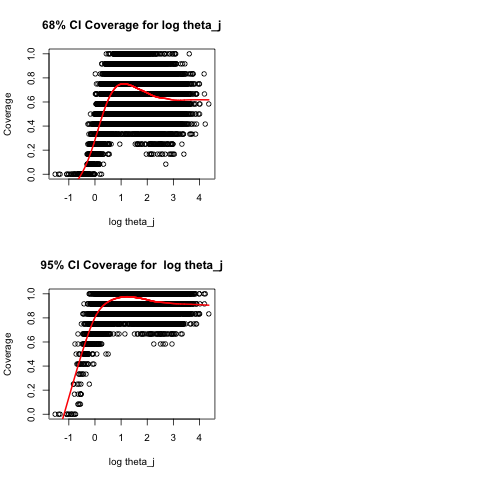
\includegraphics[scale=1, trim = 0 0 200 0]{keskici_wxiao_ps2_task3_plot1.png}
\end{figure}

\begin{figure}[h!]
  \caption{Task 3 coverage plots for $log(\theta_{j}$)'s : $\mu = 2.5$, $\sigma^2 = 1.3^2$}
  \centering
	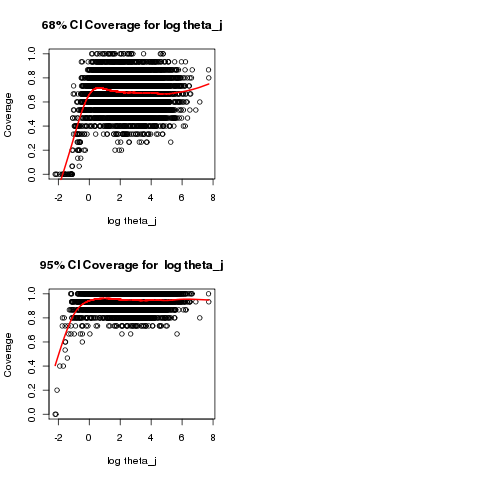
\includegraphics[scale=1, trim = 0 0 200 0]{keskici_wxiao_ps2_task3_plot2.png}
\end{figure}

\begin{figure}[h!]
  \caption{Task 3 coverage plots for $log(\theta_{j}$)'s : $\mu = 5.2$, $\sigma^2 = 1.3^2$}
  \centering
	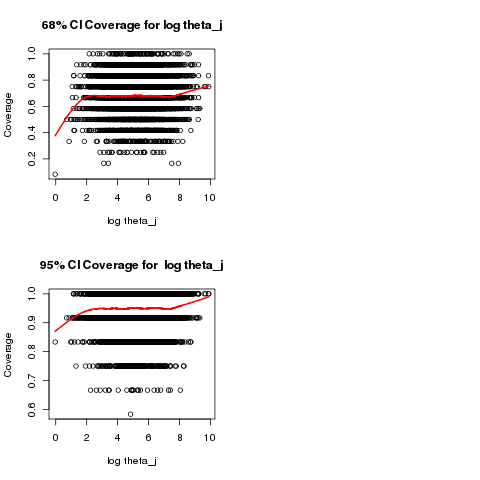
\includegraphics[scale=1, trim = 0 0 200 0]{keskici_wxiao_ps2_task3_plot3.png}
\end{figure}

\begin{figure}[h!]
  \caption{Task 3 coverage plots for $log(\theta_{j}$)'s : $\mu = 4.9$, $\sigma^2 = 1.6^2$}
  \centering
	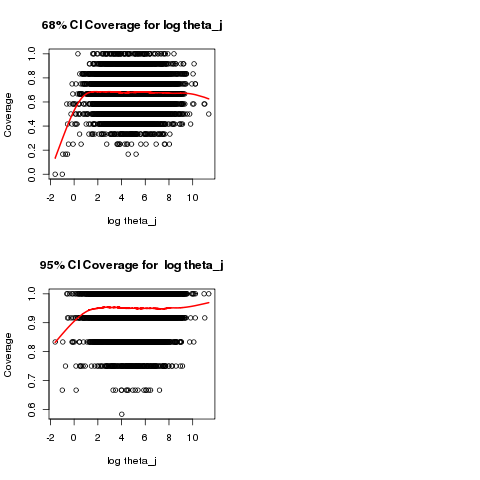
\includegraphics[scale=1, trim = 0 0 200 0]{keskici_wxiao_ps2_task3_plot4.png}
\end{figure}

%%%%%%%%%%%%%%%%%%%%%%%%%%%%%%%%%%%%%%%%%%%%%%%%%%%%%%%%%%%
\begin{figure}[h!]
  \caption{Task 4 coverage plots for $log(\theta_{j}$)'s : $\mu = 1.6$, $\sigma^2 = 0.7^2$}
  \centering
	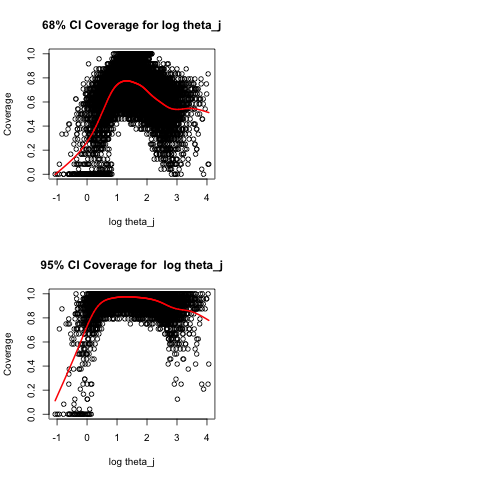
\includegraphics[scale=1, trim = 0 0 200 0]{keskici_wxiao_ps2_task4_plot1.png}
\end{figure}

\begin{figure}[h!]
  \caption{Task 4 coverage plots for $log(w_{j}$)'s : $\mu = 1.6$, $\sigma^2 = 0.7^2$}
  \centering
	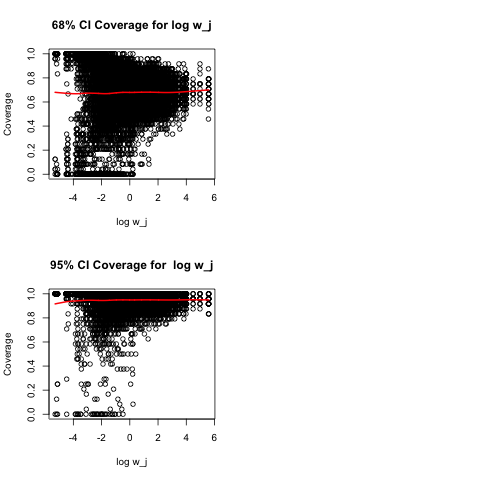
\includegraphics[scale=1, trim = 0 0 200 0]{keskici_wxiao_ps2_task4_plot2.png}
\end{figure}

\begin{figure}[h!]
  \caption{Task 4 coverage plots for $log(\theta_{j}$)'s : $\mu = 2.5$, $\sigma^2 = 1.3^2$}
  \centering
	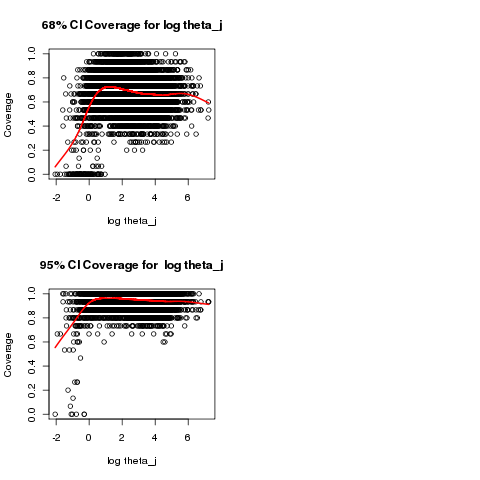
\includegraphics[scale=1, trim = 0 0 200 0]{keskici_wxiao_ps2_task4_plot3.png}
\end{figure}

\begin{figure}[h!]
  \caption{Task 4 coverage plots for $log(w_{j}$)'s : $\mu = 2.5$, $\sigma^2 = 1.3^2$}
  \centering
	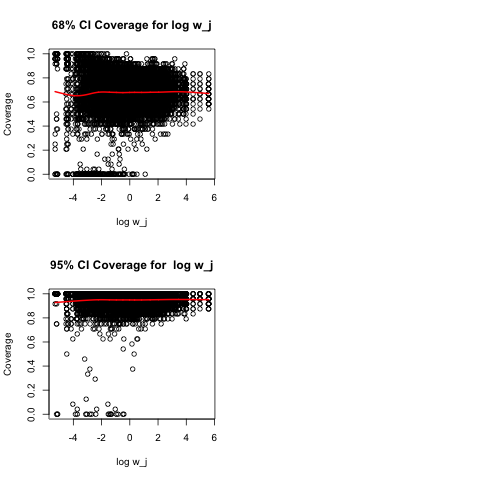
\includegraphics[scale=1, trim = 0 0 200 0]{keskici_wxiao_ps2_task4_plot4.png}
\end{figure}


\begin{figure}[h!]
  \caption{Task 4 coverage plots for $log(\theta_{j}$)'s : $\mu = 5.2$, $\sigma^2 = 1.3^2$}
  \centering
	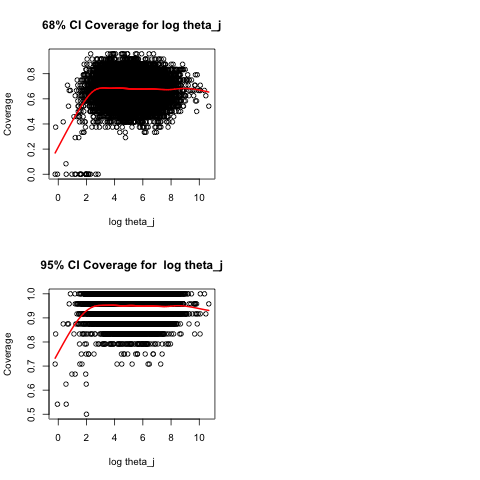
\includegraphics[scale=1, trim = 0 0 200 0]{keskici_wxiao_ps2_task4_plot5.png}
\end{figure}

\begin{figure}[h!]
  \caption{Task 4 coverage plots for $log(w_{j}$)'s : $\mu = 5.2$, $\sigma^2 = 1.3^2$}
  \centering
	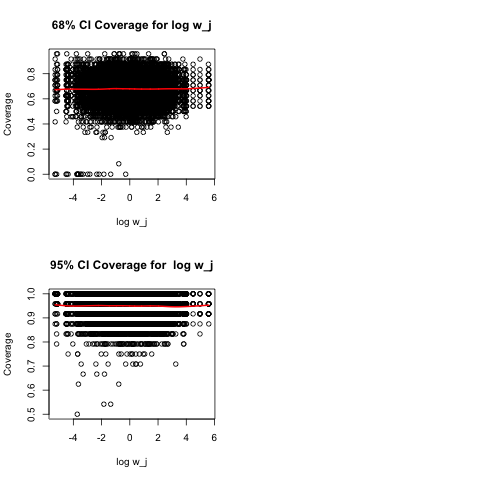
\includegraphics[scale=1, trim = 0 0 200 0]{keskici_wxiao_ps2_task4_plot6.png}
\end{figure}


\begin{figure}[h!]
  \caption{Task 4 coverage plots for $log(\theta_{j}$)'s : $\mu = 4.9$, $\sigma^2 = 1.6^2$}
  \centering
	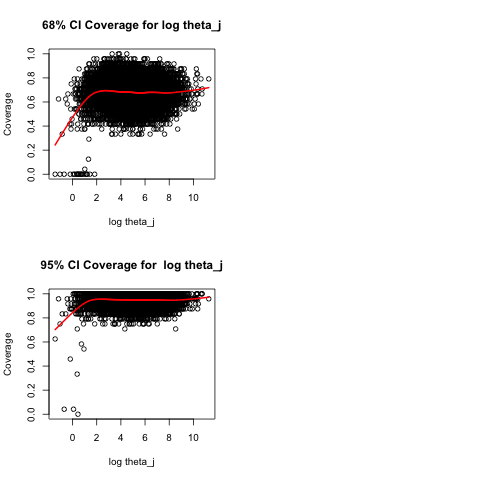
\includegraphics[scale=1, trim = 0 0 200 0]{keskici_wxiao_ps2_task4_plot7.png}
\end{figure}

\begin{figure}[h!]
  \caption{Task 4 coverage plots for $log(w_{j}$)'s : $\mu = 4.9$, $\sigma^2 = 1.6^2$}
  \centering
	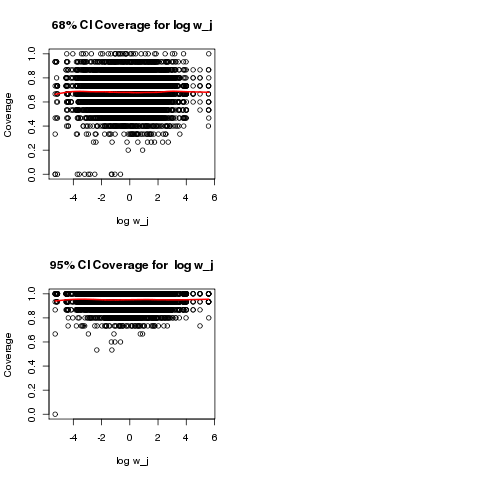
\includegraphics[scale=1, trim = 0 0 200 0]{keskici_wxiao_ps2_task4_plot8.png}
\end{figure}

%%%%%%%%%%%%%%%%%%%%%%%%%%%%%%%%%%%%%%%%%%%%%%%%%%%%%%%%%%
\begin{figure}[h!]
  \caption{Task 5 coverage plots for $log(\theta_{j}$)'s : $x_0 = 1.6$, $m = 0, b = 1.3$}
  \centering
	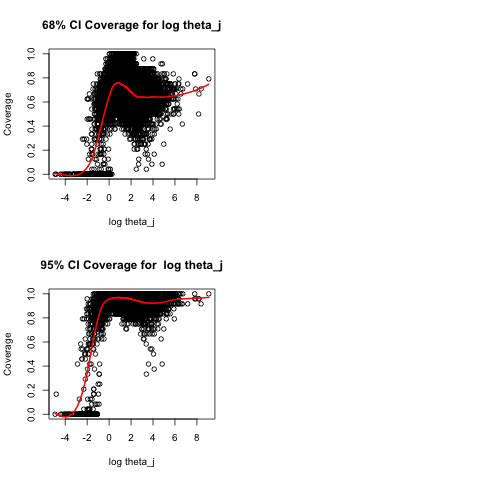
\includegraphics[scale=1, trim = 0 0 200 0]{keskici_wxiao_ps2_task5_plot1.png}
\end{figure}

\begin{figure}[h!]
  \caption{Task 5 coverage plots for $log(w_{j}$)'s : $x_0 = 1.6$, $m = 0, b = 1.3$}
  \centering
	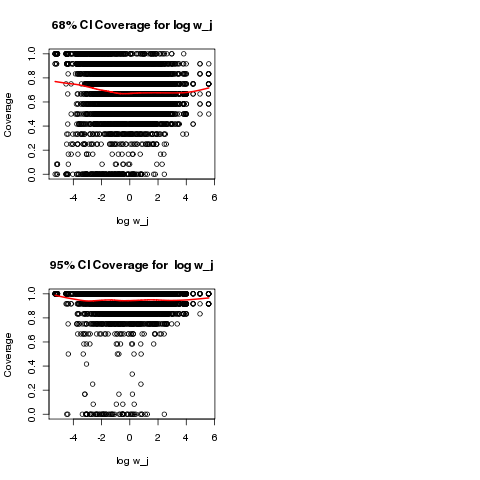
\includegraphics[scale=1, trim = 0 0 200 0]{keskici_wxiao_ps2_task5_plot2.png}
\end{figure}

\begin{figure}[h!]
  \caption{Task 5 coverage plots for $log(\theta_{j}$)'s : $x_0 = 1.6$, $m = -0.7, b = 1.3$}
  \centering
	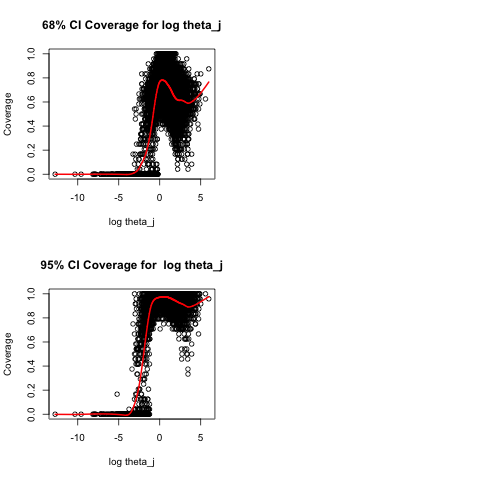
\includegraphics[scale=1, trim = 0 0 200 0]{keskici_wxiao_ps2_task5_plot3.png}
\end{figure}

\begin{figure}[h!]
  \caption{Task 5 coverage plots for $log(w_{j}$)'s : $x_0 = 1.6$, $m = -0.7, b = 1.3$}
  \centering
	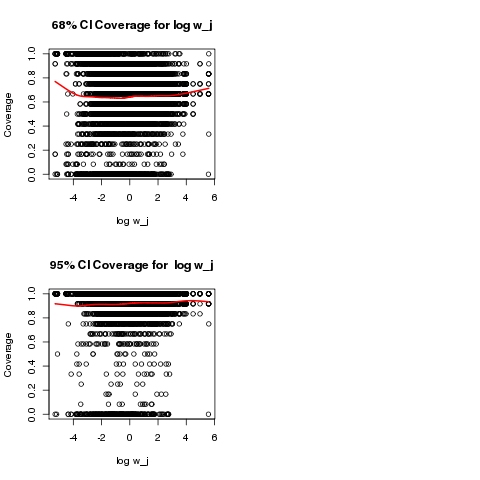
\includegraphics[scale=1, trim = 0 0 200 0]{keskici_wxiao_ps2_task5_plot4.png}
\end{figure}

\begin{figure}[h!]
  \caption{Task 5 coverage plots for $log(\theta_{j}$)'s : $x_0 = 1.6$, $m = -.7, b = 1.3$}
  \centering
	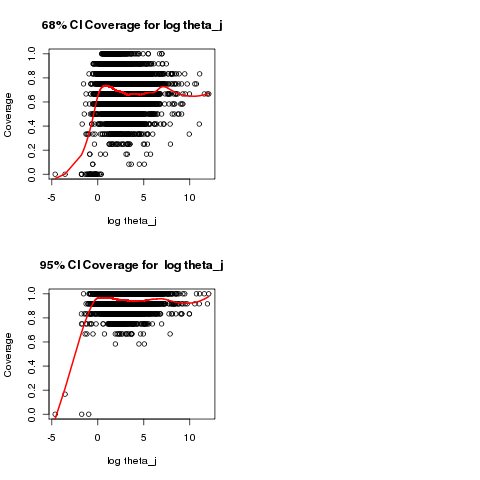
\includegraphics[scale=1, trim = 0 0 200 0]{keskici_wxiao_ps2_task5_plot5.png}
\end{figure}

\begin{figure}[h!]
  \caption{Task 5 coverage plots for $log(w_{j}$)'s : $x_0 = 1.6$, $m = 0.7, b = 1.3$}
  \centering
	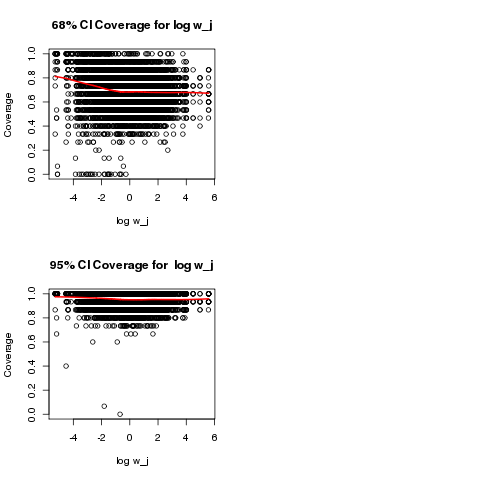
\includegraphics[scale=1, trim = 0 0 200 0]{keskici_wxiao_ps2_task5_plot6.png}
\end{figure}
\clearpage

\begin{figure}[h!]
  \caption{Task 5 coverage plots for $log(\theta_{j}$)'s : $x_0 = 1.6$, $m = 0, b = 2.6$}
  \centering
	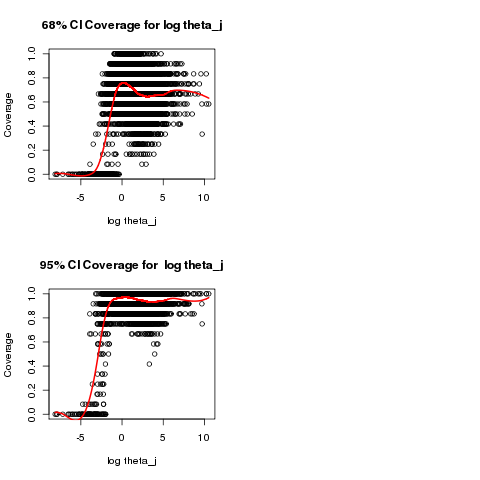
\includegraphics[scale=1, trim = 0 0 200 0]{keskici_wxiao_ps2_task5_plot7.png}
\end{figure}

\begin{figure}[h!]
  \caption{Task 5 coverage plots for $log(w_{j}$)'s : $x_0 = 1.6$, $m = 0, b = 2.6$}
  \centering
	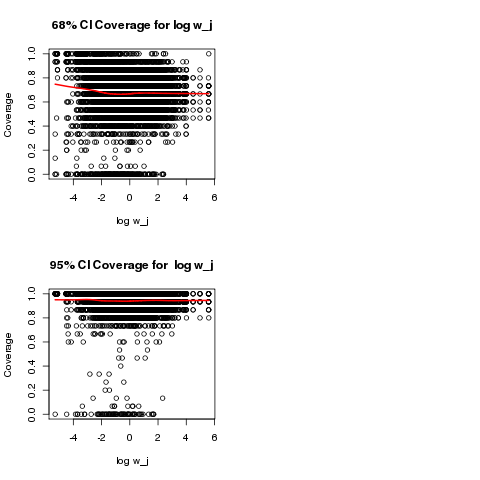
\includegraphics[scale=1, trim = 0 0 200 0]{keskici_wxiao_ps2_task5_plot8.png}
\end{figure}







\end{document}
